\section{Cân bằng trong dung dịch nước}
\begin{Muctieu}
	\begin{itemize}
		\item  Nêu được khái niệm sự điện li, chất điện li, chất không điện li.
		\item  Trình bày được thuyết Brønsted - Lowry (Bron-stêt - Lau-ri) về acid - base.
		\item  Nêu được khái niệm và ý nghĩa của pH trong thực tiễn (liên hệ giá trị pH ở các bộ phận trong cơ thể với sức khoẻ con người, pH của đất, nước tới sự phát triển của động thực vật, ...).
		\item  Viết được biểu thức tính pH và biết cách sử dụng các chất chỉ thị để xác định pH (môi trường acid, base, trung tính) bẳng các chất chỉ thị phổ biến như giấy chi thị màu, quỳ tím, phenolphthalein, ...
		\item  Nêu được nguyên tắc xác định nồng độ acid, base mạnh bằng phương pháp chuẩn độ.
		\item  Thực hiện được thí nghiệm chuẩn độ acid - base: Chuẩn độ dung dịch base mạnh (sodium hydroxide) bằng dung dich acid mạnh (hydrochloric acid).
		\item  Trình bày được ý nghĩa thực tiễn cân bằng trong dung dịch nước của ion $\mathrm{Al}^{3+}, \mathrm{Fe}^{3+}$ $\mathrm{Và}_{\mathrm{Cl}} \mathrm{CO}_3^{2-}$.
	\end{itemize}
\end{Muctieu}
\subsection{Nội dung bài học}
\begin{kd}
	\immini{Có một anh kĩ sư nông nghiệp trồng cà chua. Anh ấy nhận thấy cây cà chua của mình không phát triển tốt như mong đợi. Sau khi tìm hiểu, anh ấy biết rằng cà chua thích hợp với đất có độ pH từ $6{,}0$ đến $6{,}8$. Anh ấy đo pH của đất trong vườn và thấy nó là $5{,}5$.
		Câu hỏi đặt ra là:
		\begin{itemize}
			\item Tại sao độ pH của đất lại quan trọng đối với sự phát triển của cây trồng?
			\item Điều gì khiến độ pH của đất thay đổi?
			\item Làm thế nào để anh kĩ sư nông nghiệp có thể điều chỉnh pH của đất?
		\end{itemize}
		}{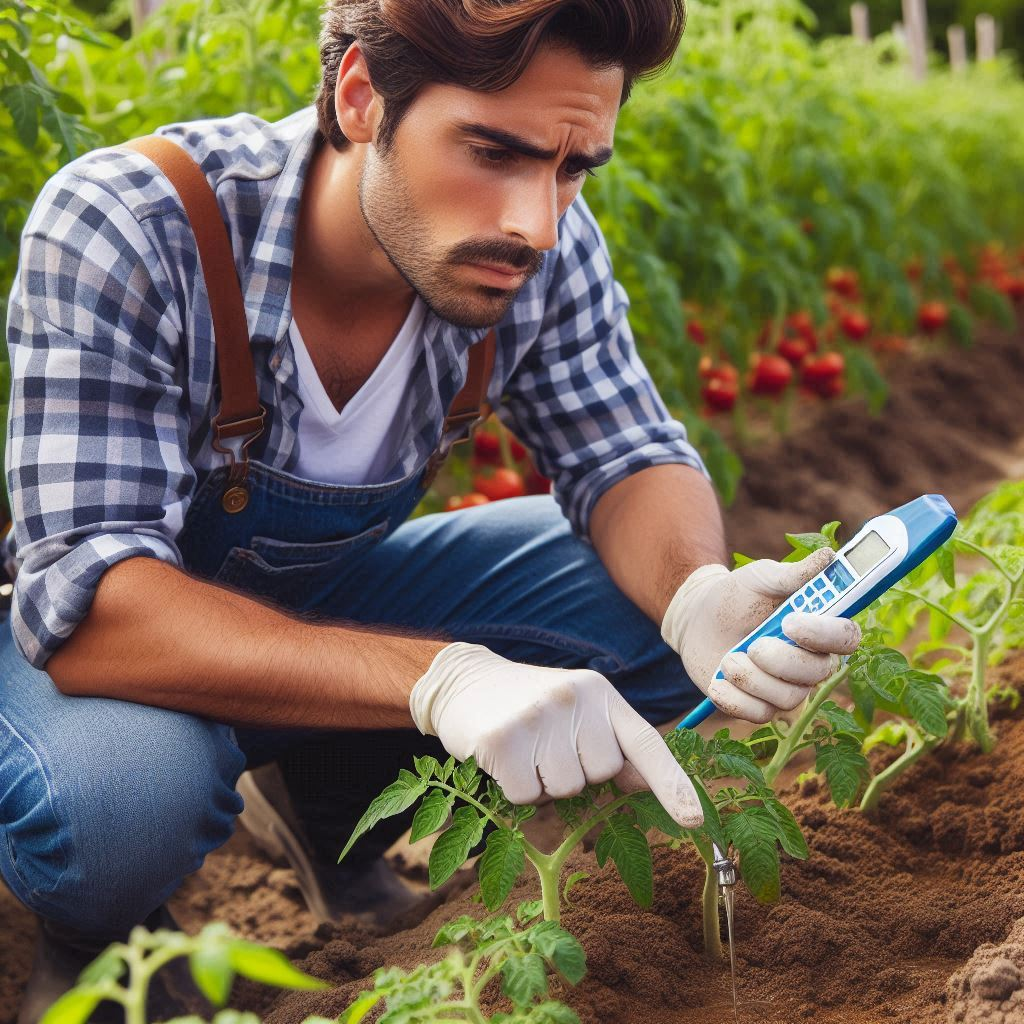
\includegraphics[width=5cm]{Images/anhhoa11/dopH.jpg}}
		Để trả lời những câu hỏi này, chúng ta cần hiểu về cân bằng axit-bazơ trong dung dịch, đặc biệt là trong môi trường đất. Đất là một hệ thống phức tạp, trong đó có nhiều phản ứng hóa học xảy ra đồng thời, bao gồm cả các phản ứng cân bằng.
\end{kd}
\subsubsection{Sự điện li}
\Noibat[\maunhan]{Hiện tượng điện li}
\Noibat[][][\faApple]{Tìm hiểu về sự điện li}
\begin{figure}[!htp]
	\begin{hopdongian}[\mauphu]
		{\indam[\mauphu]{\faAsterisk\;Thí nghiệm về sự điện li}
			\begin{itemize}
				\item \textbf{Chuẩn bị hóa chất:} Kim loại: $Al$, $Cu$; muối: $NaCl$, $CaCl_2$, $CuSO_4$; hạt nhựa PVC, đường, rượu etylic, silic dioxit.
				\item \textbf{Cách tiến hành:}
				\begin{itemize}
					\item Thí nghiệm 1: Đặt điện cực tiếp xúc trực tiếp với các chất trước khi cho nước cất vào.
					\item Thí nghiệm 2: Đặt điện cực tiếp xúc với nước sau khi rót nước vào và khuấy đều.
				\end{itemize}
				Quan sát hiện tượng.
			\end{itemize}
		}
		\begin{center}
			\begin{subfigure}[b]{0.23\textwidth}
				\centering
				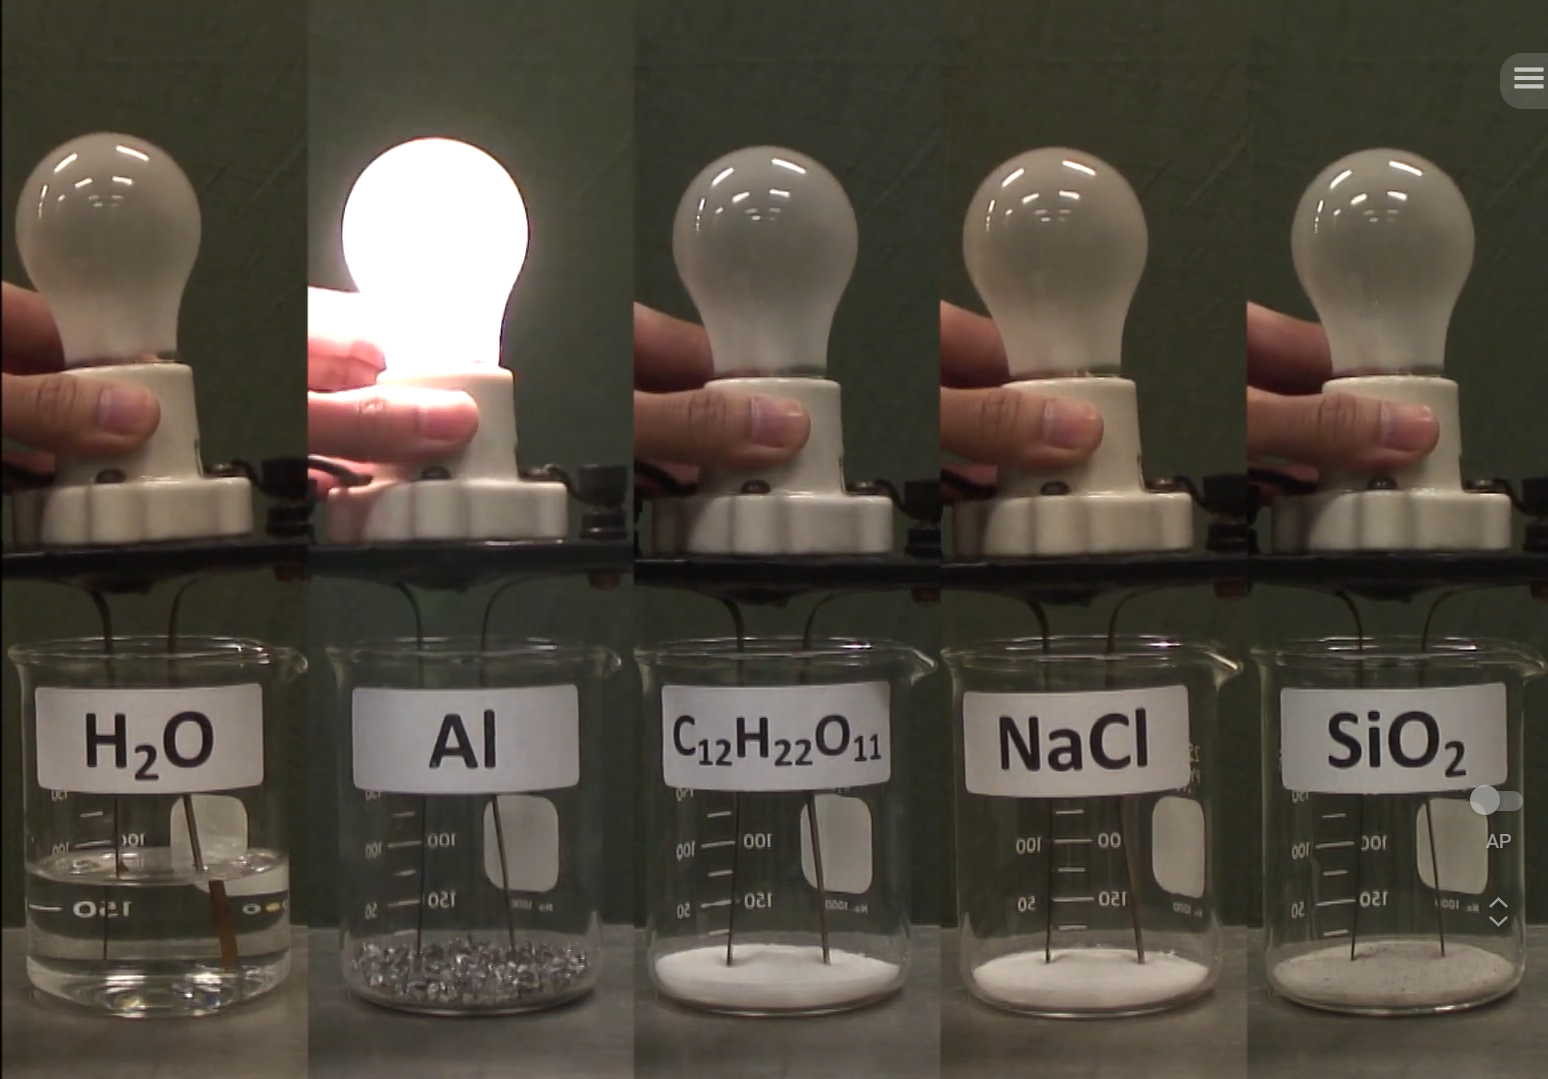
\includegraphics[height=0.7\textwidth]{Images/anhhoa11/dodandien_1.png}
				\caption{Trước khi rót nước vào}
				\label{subfig:TNsudienli1}
			\end{subfigure}
			\begin{subfigure}[b]{0.23\textwidth}
				\centering
				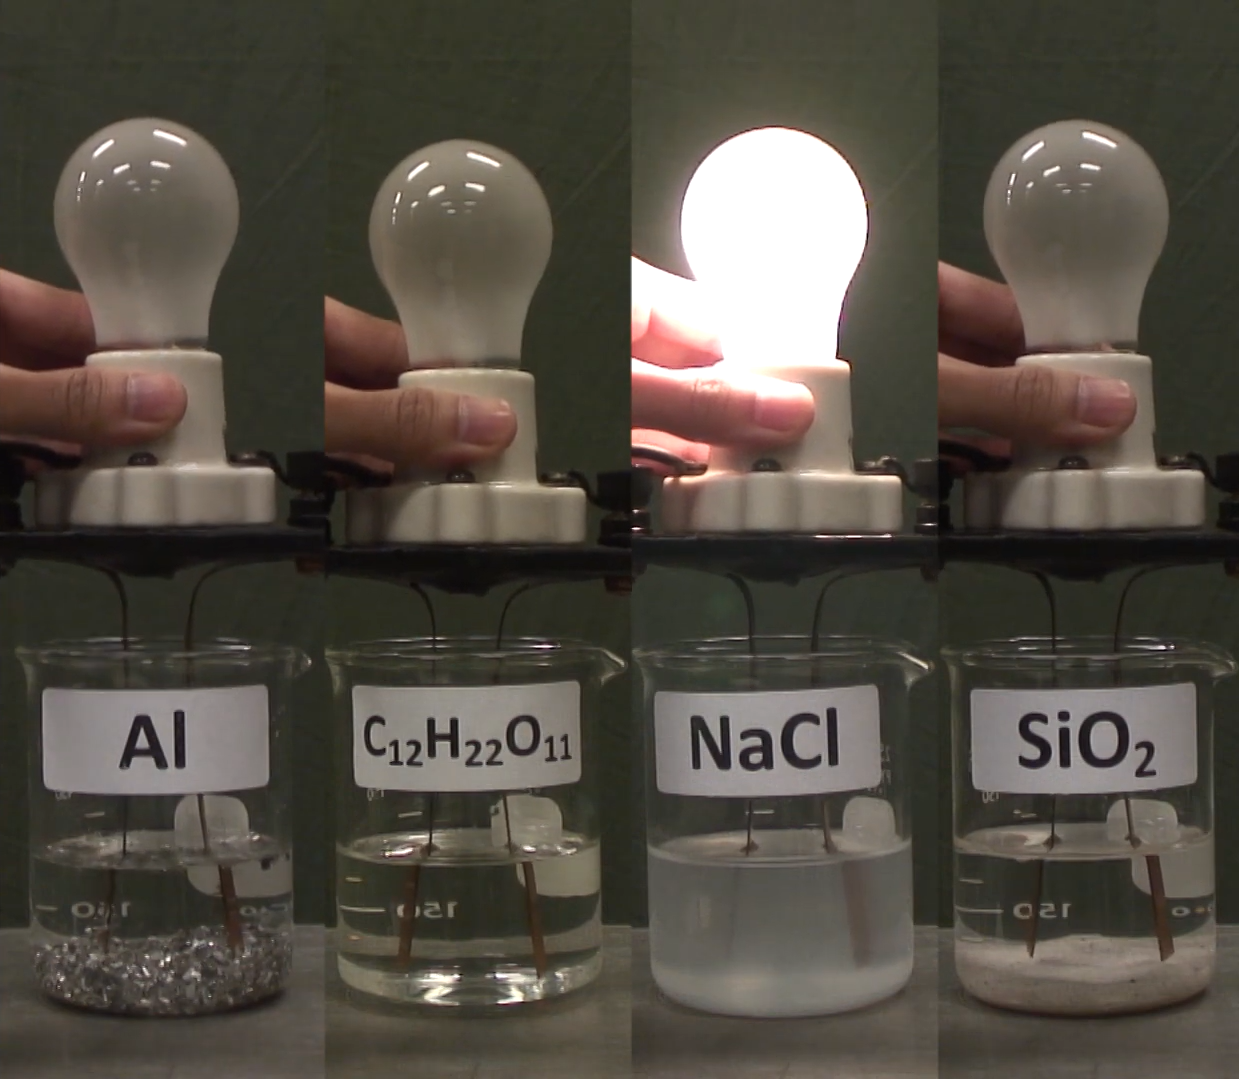
\includegraphics[height=0.7\textwidth]{Images/anhhoa11/dodandien_2.png}
				\caption{Đã rót nước và khuấy}
				\label{subfig:TNsudienli2}
			\end{subfigure}
			\hspace*{0.5cm}
			\begin{subfigure}[b]{0.23\textwidth}
				\centering
				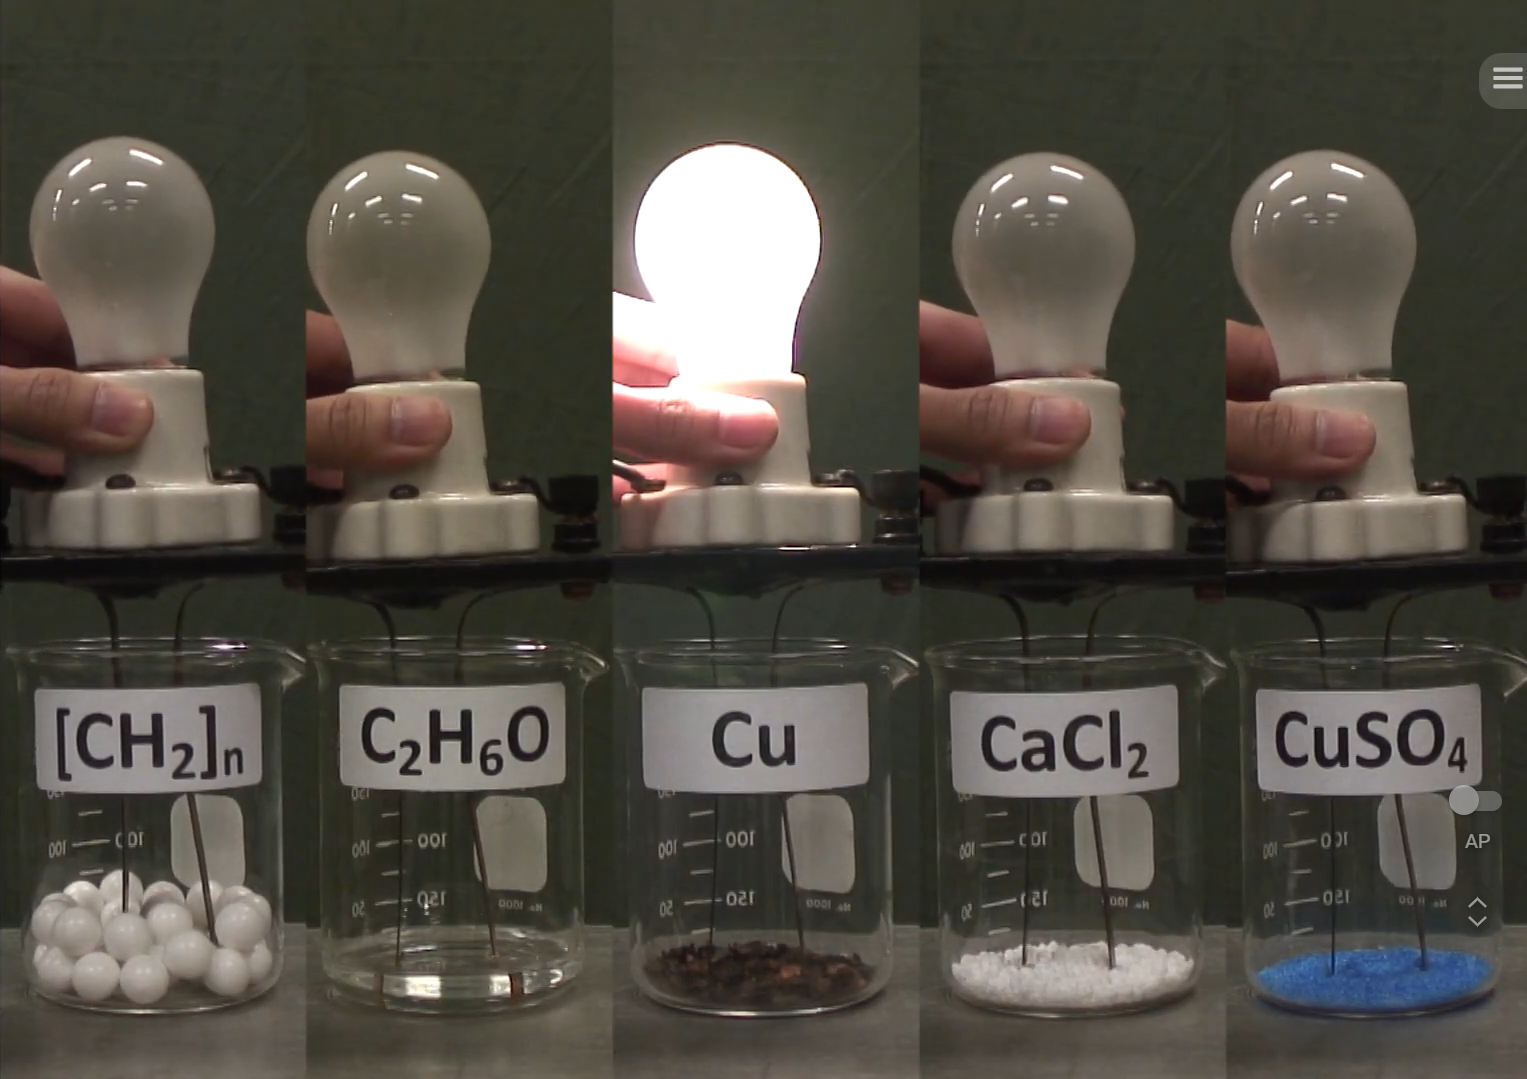
\includegraphics[height=0.7\textwidth]{Images/anhhoa11/dodandien_3.png}
				\caption{Trước khi rót nước vào}
				\label{subfig:TNsudienli3}
			\end{subfigure}
			\hspace*{0.25cm}
			\begin{subfigure}[b]{0.23\textwidth}
				\centering
				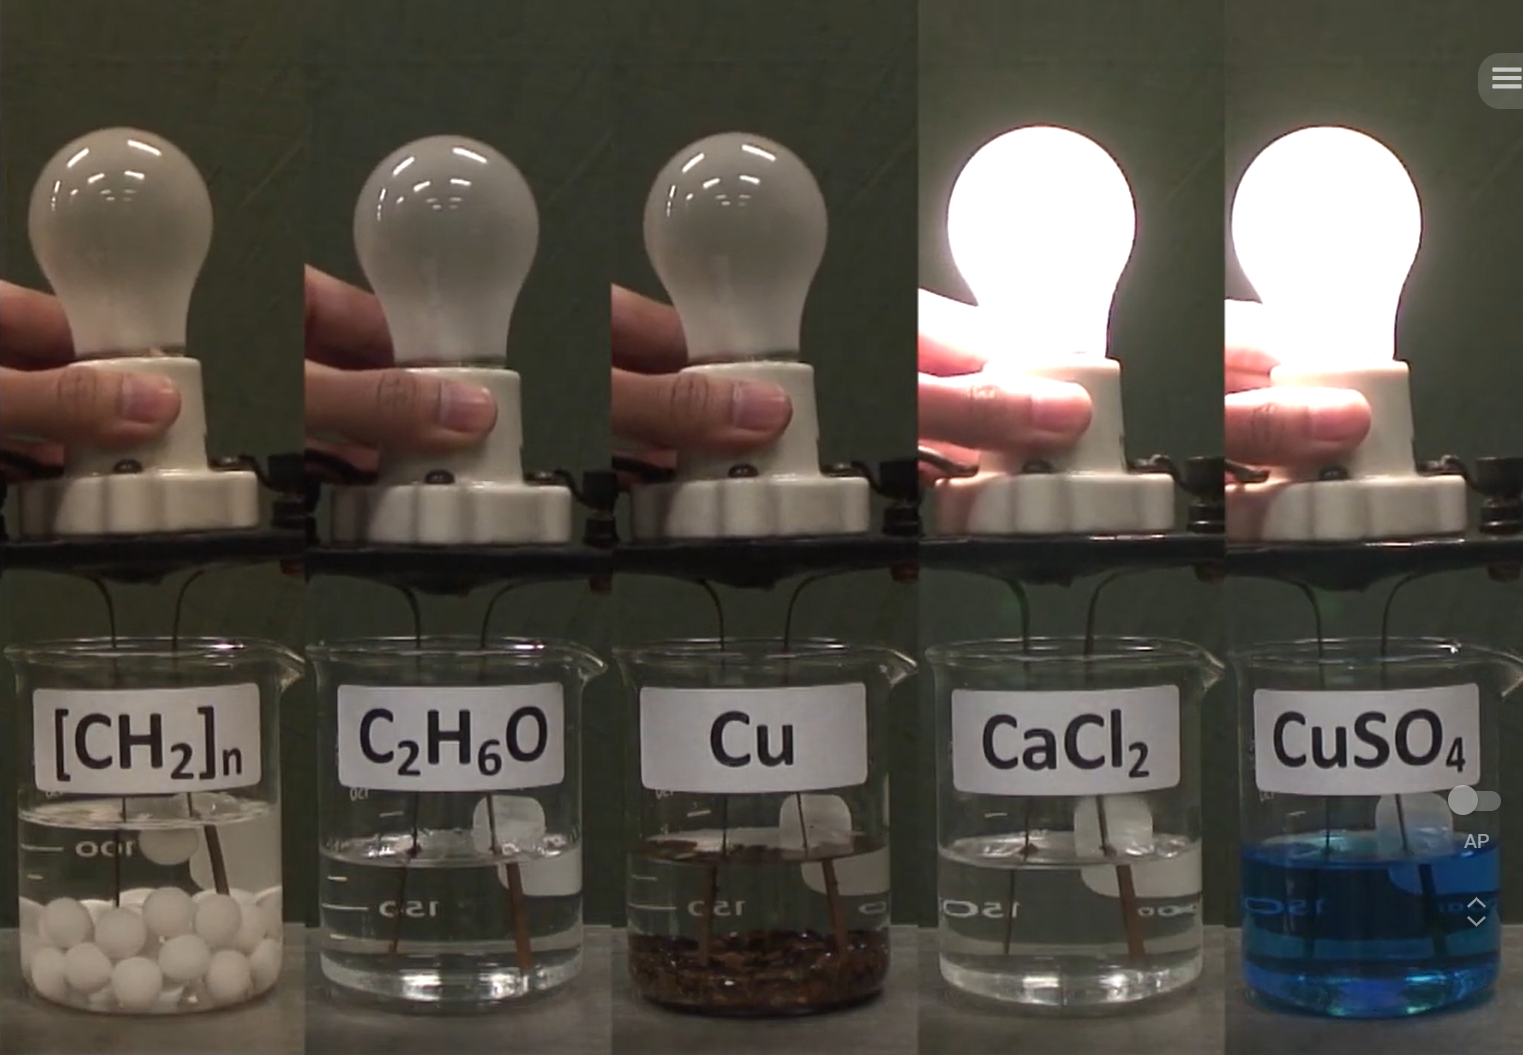
\includegraphics[height=0.7\textwidth]{Images/anhhoa11/dodandien_4.png}
				\caption{Đã cho nước và khuấy}
				\label{subfig:TNsudienli4}
			\end{subfigure}
			\caption{Thí nghiệm về sự điện li}
			\label{fig:TNsudienli}
		\end{center}
	\end{hopdongian}
\end{figure}
\begin{hoivadap}
	\begin{cauhoi}
		Quan sát ở hình \ref{fig:TNsudienli} hãy trả lời các câu hỏi sau:
	    \begin{enumerate}[(1)]
	    	\item Trước khỉ rót nước vào (thí nghiệm 1), bóng đèn có sáng khi nhúng cặp điện cực vào các chất nào? Tại sao?
	    	Đối với các chất không làm sáng bóng đèn trong thí nghiệm 1, bạn có nhận xét gì về trạng thái của chúng (rắn, lỏng, khí)?
	    	\item Sau khi hòa tan các chất vào nước và khuấy đều (thí nghiệm 2), bóng đèn có sáng khi nhúng cặp điện cực vào dung dịch nào? 
	    	\item So sánh kết quả của thí nghiệm 1 và thí nghiệm 2. Bạn nhận thấy điều gì khác biệt?
	    	\item Đối với các chất làm sáng bóng đèn trong thí nghiệm 2 nhưng không làm sáng trong thí nghiệm 1, điều gì đã xảy ra khi chúng được hòa tan vào nước?Theo bạn, tại sao một số chất chỉ dẫn điện khi được hòa tan vào nước?
	    	\item Nếu một chất khi hòa tan vào nước làm cho dung dịch dẫn điện, bạn nghĩ trong dung dịch đó có gì?
	    \end{enumerate}
	\end{cauhoi}
	\loigiai{%
		\begin{enumerate}[(1)]
			\item Trong thí nghiệm 1 trước khỉ rót nước vào, bóng đèn sáng khi nhúng cặp điện cực vào kim loại $Al$, $Cu$. Đây là do kim loại  có cấu trúc tinh thể với các electron tự do có thể di chuyển, cho phép dòng điện đi qua.
			Các chất không làm sáng bóng đèn như (nước cất,nhựa PVC, rượu, canxi clorua rắn, đồng sunfat khan,...) đều ở trạng thái rắn hoặc lỏng, nhưng không có cấu trúc cho phép các hạt mang điện di chuyển tự do.
			\item Trong thí nghiệm 2, sau khi hòa tan các chất vào nước và khuấy đều, bóng đèn sáng khi nhúng cặp điện cực vào dung dịch Natri clorua,canxi clorua và dung dịch đồng sunfat.
			\item So sánh kết quả của hai thí nghiệm, ta nhận thấy:
			\begin{itemize}
				\item Thí nghiệm 1: Chỉ có kim loại đồng, nhôm dẫn điện.
				\item Thí nghiệm 2: dung dịch natri clorua,canxi clorua và đồng sunfat  dẫn điện.
			\end{itemize}
			Điều này cho thấy một số chất không dẫn điện ở trạng thái rắn, nhưng lại dẫn điện khi hòa tan trong nước.
			\item Khi Natriclorua, canxi clorua và đồng sunfat được hòa tan vào nước, chúng phân li thành các ion. Các ion này có khả năng di chuyển tự do trong dung dịch, cho phép dòng điện đi qua. Một số chất chỉ dẫn điện khi hòa tan trong nước vì nước có khả năng phân li các chất thành các ion mang điện.
			\item Khi một chất hòa tan vào nước làm cho dung dịch dẫn điện, trong dung dịch đó có các ion. Các ion này là các hạt mang điện có khả năng di chuyển tự do trong dung dịch, cho phép dòng điện đi qua. Ví dụ, trong dung dịch canxi clorua, ta có các ion $Ca^{2+}$ và $Cl^-$, còn trong dung dịch đồng sunfat, ta có các ion $Cu^{2+}$ và $SO4^{2-}$.
		\end{enumerate}}
\end{hoivadap}
\begin{tomtat}
	Quá trình phân li các chất trong nước tạo thành ion được gọi là \indam{sự điện li}.
\end{tomtat}
\Noibat[\maunhan]{Chất điện li}
\Noibat[\mauphu][][\faArrowCircleORight]{Chất điện li và chất không điện li}
\\
Thí nghiệm trên cho thấy: các chất như natri clorua, canxi clorua,... tan trong nước phân li ra các ion nên chúng là chất điện li. Saccarose, ethanol,... không phân li ra các ion nên chúng là chất không điện li.
\\
Như vậy trong dung dịch $NaCl$ có chứa các ion $Na^+$ và $Cl^-$ mang điện còn ở dung dịch đường chức các phân tử đường không mang điện
\begin{equation}\label{eq:dienliNaCl}
	\mathrm{NaCl}(s) \rightarrow \mathrm{Na}^{+}(a q)+\mathrm{Cl}^{-}(a q)
\end{equation}
\begin{equation}
	\mathrm{C}_{12} \mathrm{H}_{22} \mathrm{O}_{11}(s) \rightarrow \mathrm{C}_{12} \mathrm{H}_{22} \mathrm{O}_{11}(a q)
\end{equation}
Phương trình (\ref{eq:dienliNaCl}) được gọi là \indam{phương trình điện li}
\vspace{0.25cm}
\begin{tomtat}
	 \begin{itemize}
	 	\item Những chất khi tan trong nước phân li ra các ion được gọi là \indam{chất điện li}
	 	\item Những chất khi tan trong nước không phân li thành các ion được gọi là \indam{Chất không diện li} .
	 \end{itemize}
\end{tomtat}
\Noibat[\mauphu][][\faArrowCircleORight]{Chất điện li mạnh và chất điện li yếu}
\begin{figure}[!htp]
	\begin{hopdongian}[\mauphu]
		{\indam[\mauphu]{\faAsterisk\;Thí nghiệm so sánh khả năng phân li trong nước của $HCl$ và $CH_3COOH$}\\
		- Chuẩn bị 2 dung dịch $\mathrm{HCl}$ $0{,}1\mathrm{M}$ và dung dịch $\mathrm{CH}_3\mathrm{COOH}$ $0{,}1\mathrm{M}$, cắm điện cực vào 2 dung dịch , quan sát hiện tượng xảy ra?
		}
		\begin{center}
			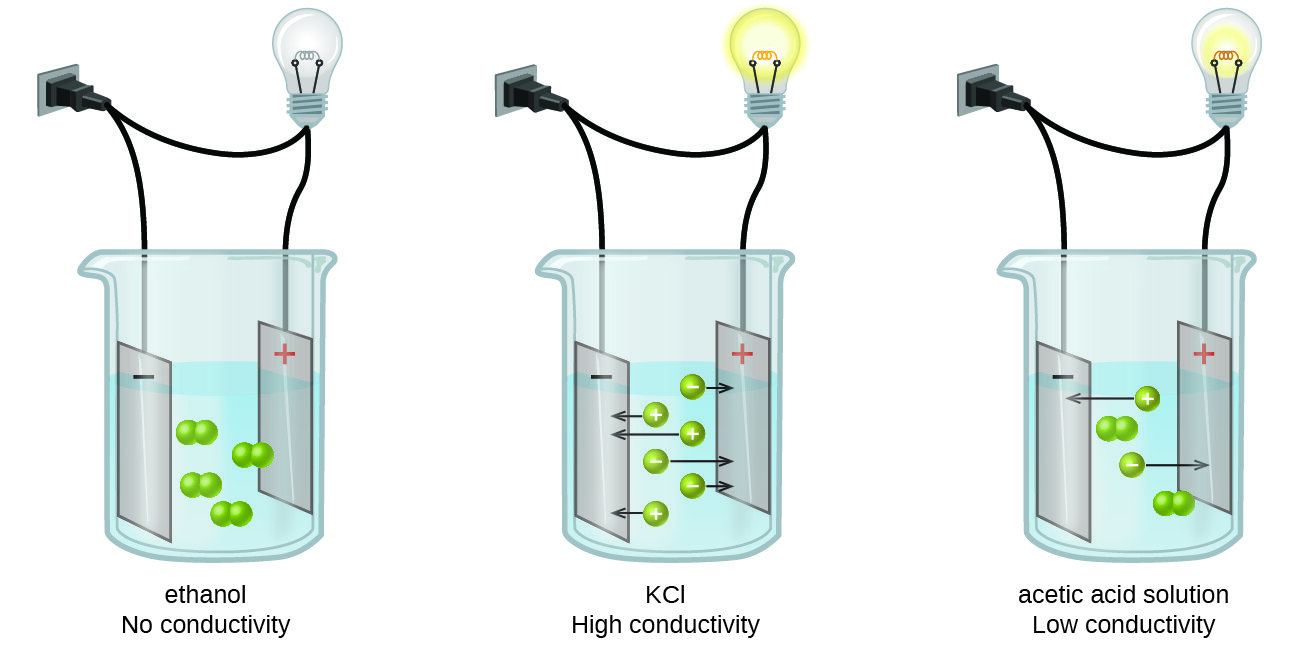
\includegraphics[width=5.5cm,trim={6cm 0cm 0cm 0cm},clip]{Images/anhhoa11/dodandien.jpg}
			\caption{Thí nghiệm so sánh khả năng phân li của $HCl$ và $CH_3COOH$}
			\label{fig:ssdodienli}
		\end{center}
	\end{hopdongian}
\end{figure}
\begin{hoivadap}
	\begin{cauhoi}
		Quan sát và nêu hiện tượng của thí nghiệm?Giải thích
	\end{cauhoi}
		\loigiai{%
		\\
		\textbf{Hiện tượng}:
		Cả hai dung dịch đều dẫn điện, nhưng dung dịch $\mathrm{HCl} 0,1 \mathrm{M}$ dẫn điện tốt hơn dung dịch $\mathrm{CH}_3\mathrm{COOH} 0,1 \mathrm{M}$.\\
		\textbf{Giải thích}:
	\begin{itemize}
		\item Cả $\mathrm{HCl}$ và $\mathrm{CH}_3\mathrm{COOH}$ đều là axit, khi hòa tan trong nước sẽ điện ly tạo ra các ion:
		\begin{align*}
		\mathrm{HCl} \rightarrow \mathrm{H}^+ + \mathrm{Cl}^-\\
		\mathrm{CH}_3\mathrm{COOH} \rightleftharpoons \mathrm{CH}_3\mathrm{COO}^- + \mathrm{H}^+
		\end{align*}
		\item Độ dẫn điện của dung dịch phụ thuộc vào số lượng ion trong dung dịch. Dung dịch có nhiều ion hơn sẽ dẫn điện tốt hơn.Khi nhúng điện cực vào dung dịch $HCl$ đèn sáng mạnh hơn so với dung dịch $CH_3COOH$, điều đó chứng tỏ $HCl$ khi hòa tan vào nước phân li ra nhiều ion hơn so với $CH_3COOH$
		\item \textbf{Kết luận:} Dung dịch $\mathrm{HCl} 0{,}1 \mathrm{M}$ dẫn điện tốt hơn dung dịch $\mathrm{CH}_3\mathrm{COOH} 0{,}1 \mathrm{M}$ vì $\mathrm{HCl}$ là axit mạnh, điện ly hoàn toàn, tạo ra nhiều ion hơn trong dung dịch so với $\mathrm{CH}_3\mathrm{COOH}$ - một axit yếu chỉ điện ly một phần.
	\end{itemize}
	}
\end{hoivadap}
\vspace*{0.25cm}
\begin{tomtat}
	Dựa vào mức độ phân li thành các ion, chất điện li được chia thành hai loại:
	\begin{enumerate}
	\item \indam{Chất điện li mạnh} là chất khi tan trong nước, hầu hết các phân tử chất tan đều phân li ra ion. Các chất điện li mạnh thường gặp là:
\begin{itemize}
		\item \textbf{Các acid mạnh:} $\mathrm{HCl}, \mathrm{HNO}_3, \mathrm{H}_2 \mathrm{SO}_4, \ldots$
		\item \textbf{Các base mạnh:} $\mathrm{NaOH}, \mathrm{KOH}, \mathrm{Ca}(\mathrm{OH})_2, \mathrm{Ba}(\mathrm{OH})_2, \ldots$
		\item \textbf{Hầu hết các muối.}
		
	Quá trình phân li của chất điện li mạnh xảy ra gần như hoàn toàn và được biểu diễn bằng \textbf{mũi tên một chiều}.
	\[
	\begin{aligned}
		& \mathrm{HNO}_3 \longrightarrow \mathrm{H}^{+}+\mathrm{NO}_3^{-} \\
		& \mathrm{NaOH} \longrightarrow \mathrm{Na}^{+}+\mathrm{OH}^{-} \\
		& \mathrm{Na}_2 \mathrm{CO}_3 \longrightarrow 2 \mathrm{Na}^{+}+\mathrm{CO}_3^{2-}
	\end{aligned}
	\]
	\end{itemize}
	\item \indam{Chất điện li yếu} là chất khi tan trong nước chỉ có một phần số phân tử chất tan phân li ra ion, phần còn lại vẫn tồn tại ở dạng phân tử trong dung dịch.
	\\
	Ví dụ: trong dung dịch $\mathrm{CH}_3 \mathrm{COOH} 0,1 \mathrm{M}$, cứ 1000 phân tử hoà tan thì chỉ có 3 phân tử phân li thành ion, còn lại tồn tại ở dạng phân tử.
	\\
	Những chất điện li yếu gồm :
	\begin{itemize}
		\item \textbf{Các acid yếu:} $\mathrm{CH}_3 \mathrm{COOH}, \mathrm{HClO}, \mathrm{HF}, \mathrm{H}_2 \mathrm{CO}_3, \ldots$  
		\item \textbf{Các base yếu:} $\mathrm{Cu}(\mathrm{OH})_2, \mathrm{Fe}(\mathrm{OH})_2, \ldots$
	\end{itemize}
	Quá trình phân li của chất điện li yếu là một phản ứng thuận nghịch và được biểu diễn bằng \textbf{hai nửa mũi tên ngược chiều nhau}
	$$
	\mathrm{CH}_3 \mathrm{COOH} \rightleftharpoons \mathrm{H}^{+}+\mathrm{CH}_3 \mathrm{COO}^{-} .
	$$
	\end{enumerate}
\end{tomtat}
\begin{hopvidu}
	\Noibat[][][\faArchive]{Cơ chế quá trình điện li}\\
	Nước đóng vai trò quan trọng trong sự điện li của một chất. Điều này được giải thích bởi nước là phân tử phân cực (các nguyên tử H mang một phần điện tích dương và nguyên tử O mang một phần điện tích âm) nên khi hoà tan một chất điện li vào nước, xuất hiện tương tác của nước với các ion. Tương tác này sẽ bứt các ion khỏi tinh thể (hoặc phân tử) đế tan vào nước.
	\begin{center}
		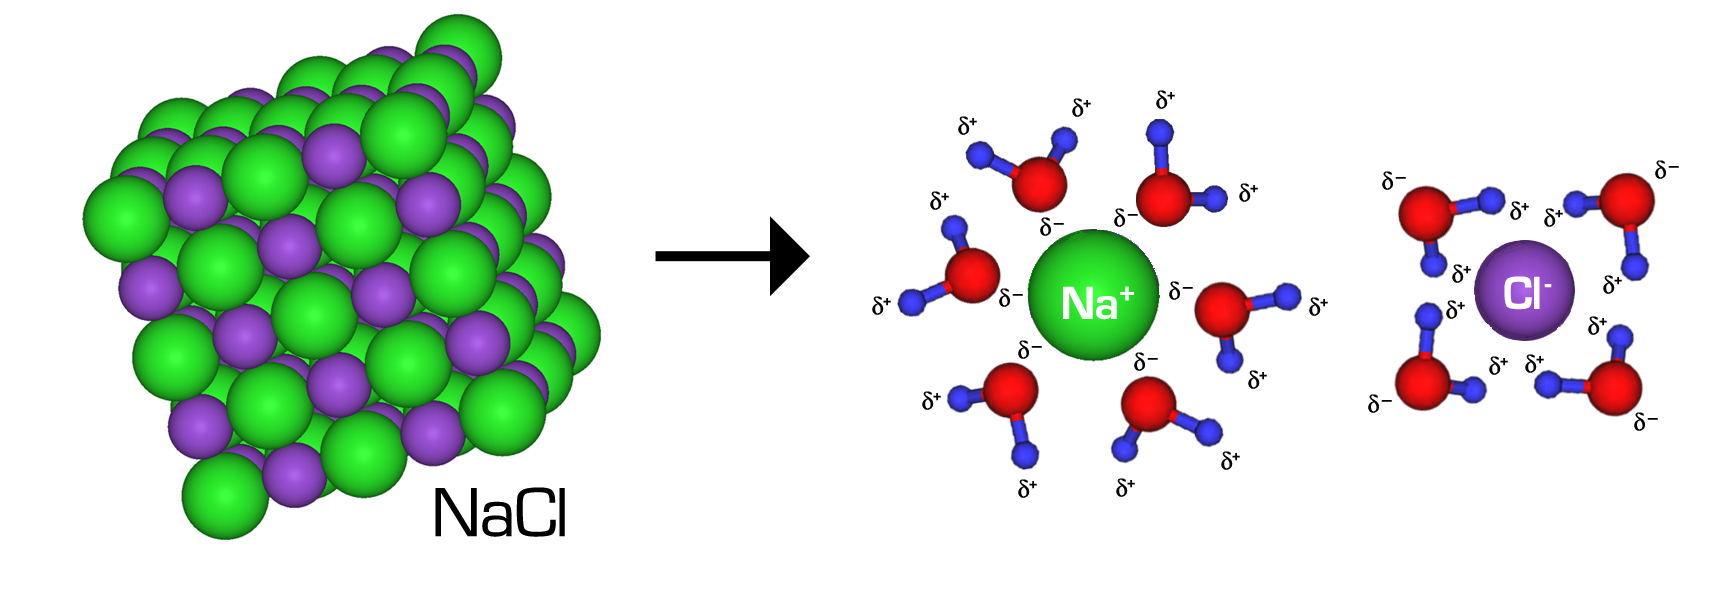
\includegraphics[height=4cm]{Images/anhhoa11/hoatanNaCl_2.jpg}
		\captionof{figure}{Quá trình điện li NaCl trong nước}
	\end{center}
\end{hopvidu}
\subsubsection{Thuyết acid-base của bronsted - lowry}
\Noibat[\maunhan]{Khái niệm acid và base theo bronsted - lowry}
%%%==============Bai_BT1==============%%%
\begin{hoivadap}
	\begin{cauhoi}
		Cho các dung dịch: $\mathrm{HCl}, \mathrm{NaOH}, \mathrm{Na_2CO_3}$.
		\begin{enumerate}
			\item Viết phương trình điện li của các chất trên.
			\item Theo khái niệm acid-base trong môn Khoa học tự nhiên ở lớp 8, trong những chất cho ở trên: Chất nào là acid? Chất nào là base?
			\item Sử dụng máy đo pH (hoặc giấy pH) xác định pH, môi trường (acid/base) của các dung dịch trên.
		\end{enumerate}
	\end{cauhoi}
	\loigiai{
		\begin{enumerate}
			\item Phương trình điện li của các chất:
			\[
			\mathrm{HCl} \rightarrow \mathrm{H}^+ + \mathrm{Cl}^-
			\]
			\[
			\mathrm{NaOH} \rightarrow \mathrm{Na}^+ + \mathrm{OH}^-
			\]
			\[
			\mathrm{Na_2CO_3} \rightarrow 2\mathrm{Na}^+ + \mathrm{CO_3}^{2-}
			\]
			\item Theo khái niệm acid-base trong môn Khoa học tự nhiên ở lớp 8:
			\begin{itemize}
				\item HCl là acid vì nó giải phóng ion H\(^+\) khi hòa tan trong nước.
				\item NaOH là base vì nó giải phóng ion OH\(^-\) khi hòa tan trong nước.
				\item Na\(_2\)CO\(_3\) không phải là bazơ vì khi tan vào nước nó không phân ly ra $OH^-$.
			\end{itemize}
			\item Sử dụng máy đo pH (hoặc giấy pH) xác định:
			\begin{itemize}
				\item Dung dịch HCl: pH < 7, môi trường acid.
				\item Dung dịch NaOH: pH > 7, môi trường base.
				\item Dung dịch Na\(_2\)CO\(_3\): pH > 7, môi trường base.
			\end{itemize}
	\end{enumerate}}
\end{hoivadap}
\begin{hoivadap}
	\begin{cauhoi}
	Nếu theo quan điểm cũ, Na\(_2\)CO\(_3\) không phải là bazơ vì không phân ly ra ion OH\(^-\). Tuy nhiên, khi đo pH, ta lại thấy dung dịch Na\(_2\)CO\(_3\) có tính bazơ. Điều này có mâu thuẫn không?
	\end{cauhoi}
	\loigiai{Khái niệm acid-base đề cập ở lớp 8 chỉ đúng với dung môi nước và chưa phản ánh đầy đủ bản chất acid/base. Năm 1923, nhà hoá học người Đan Mạch J. Brønsted (Bronstết) và nhà hoá học người Anh T. Lowry (Lao-ri) đã đưa ra một định nghĩa tổng quát hơn về acid, base.}
\end{hoivadap}
\vspace{0.25cm}
\begin{tomtat}
	\indam{Thuyết Brønsted - Lowry:} \indam[\mauphu]{acid} là chất \indam[\mauphu]{cho proton} $\left(\mathrm{H}^{+}\right)$ và \indam[\mauphu]{base} là chất \indam[\mauphu]{nhận proton}. Acid và base có thể là phân tử hoặc ion.
\end{tomtat}

\begin{vidu}
	\begin{enumerate}
		\item \begin{tikzpicture}[anchor=base, baseline]
		\tikzstyle{mynode} =[
		font=\bfseries,
		anchor=base,
		align =center,
		minimum width = 1cm,
		minimum height = .65cm
		]
		%%%==================%%%
		\tikzstyle{mymatrix} = [
		matrix of nodes,
		nodes in empty cells,
		nodes={mynode},
		column sep=-\pgflinewidth,
		row sep = -\pgflinewidth
		]
		%%%=======================================================%%%
		\matrix(m) [mymatrix]{
		$\mathsf{\color{\maunhan}HCl}$	& + & $\mathsf{H_2O}$ & $\xleftrightarrow$ & $\mathsf{\color{\maunhan}H_3O^+}$ &  + & $\mathsf{Cl^-}$\\
		};
		\path [draw,-stealth,line width=1pt] ([xshift=-0.25cm]m-1-1.south) |-([yshift=-0.5cm]m-1-2.south)node[above]{$H^+$}-|(m-1-3.south) ;
	\end{tikzpicture}
	\\
	Trong phản ứng trên: HCl cho $\mathrm{H}^{+}, \mathrm{HCl}$ là acid; $\mathrm{H}_2 \mathrm{O}$ nhận $\mathrm{H}^{+}, \mathrm{H}_2 \mathrm{O}$ là base.
	%%%
	\item \begin{tikzpicture}[anchor=base, baseline]
		\tikzstyle{mynode} =[
		font=\bfseries,
		anchor=base,
		align =center,
		minimum width = 1cm,
		minimum height = .65cm
		]
		%%%==================%%%
		\tikzstyle{mymatrix} = [
		matrix of nodes,
		nodes in empty cells,
		nodes={mynode},
		column sep=-\pgflinewidth,
		row sep = -\pgflinewidth
		]
		%%%=======================================================%%%
		\matrix(m) [mymatrix]{
			$\mathsf{NH_3}$	& + & $\mathsf{\color{\maunhan}H_2O}$ & $\xleftrightarrow$ & $\mathsf{\color{\maunhan}NH_4^+}$ &  + & $\mathsf{OH^-}$\\
		};
		\path [draw,<-,line width=1pt,>=stealth] ([xshift=-0.25cm]m-1-1.south) |-([yshift=-0.5cm]m-1-2.south)node[above,xshift=-0.25cm]{$H^+$}-|([xshift=-0.25cm]m-1-3.south) ;
	\end{tikzpicture}
	\\
	Trong phản ứng trên: $H_2O$ cho $\mathrm{H}^{+}, \mathrm{H_2O}$ là acid; $\mathrm{NH}_3$ nhận $\mathrm{H}^{+}$, $\mathrm{NH}_3$ là base.
	%%%
		%%%
	\item \begin{tikzpicture}[anchor=base, baseline]
		\tikzstyle{mynode} =[
		font=\bfseries,
		anchor=base,
		align =center,
		minimum width = 1cm,
		minimum height = .65cm
		]
		%%%==================%%%
		\tikzstyle{mymatrix} = [
		matrix of nodes,
		nodes in empty cells,
		nodes={mynode},
		column sep=-\pgflinewidth,
		row sep = -\pgflinewidth
		]
		%%%=======================================================%%%
		\matrix(m) [mymatrix]{
			$\mathsf{CO_3^{2-}}$	& + & $\mathsf{\color{\maunhan}H_2O}$ & $\xleftrightarrow$ & $\mathsf{\color{\maunhan}HCO_3^-}$ &  + & $\mathsf{OH^-}$\\
		};
		\path [draw,<-,line width=1pt,>=stealth] ([xshift=-0.25cm]m-1-1.south) |-([yshift=-0.5cm]m-1-2.south)node[above,xshift=-0.25cm]{$H^+$}-|([xshift=-0.25cm]m-1-3.south) ;
		\path [draw,->,line width=1pt,>=stealth] ([xshift=-0.45cm]m-1-5.north) |-([yshift=0.5cm]m-1-6.north)node[below,xshift=-0.35cm]{$H^+$}-|([xshift=-0.25cm]m-1-7.north) ;
	\end{tikzpicture}
	\\
	Trong phản ứng thuận, $\mathrm{CO}_3^{2-}$ nhận $\mathrm{H}^{+}$của $\mathrm{H}_2 \mathrm{O}, \mathrm{CO}_3^{2-}$ là base, $\mathrm{H}_2 \mathrm{O}$ là acid. Trong phản ứng nghịch, ion $\mathrm{HCO}_3^{-}$là acid, ion $\mathrm{OH}^{-}$là base.
	\end{enumerate}
\end{vidu}
%%%==============Bai_BT1==============%%%
\begin{hoivadap}
	\begin{cauhoi}
		Dựa vào thuyết acid-base của Brønsted-Lowry, hãy xác định chất nào là acid, chất nào là base trong các phản ứng sau:
		\begin{enumerate}
			\item $\mathrm{CH_3COOH} + \mathrm{H_2O} \rightleftharpoons \mathrm{CH_3COO^{-}} + \mathrm{H_3O^{+}}$
			\item $\mathrm{S^{2-}} + \mathrm{H_2O} \rightleftharpoons \mathrm{HS^{-}} + \mathrm{OH^{-}}$
		\end{enumerate}
	\end{cauhoi}
	\loigiai{
		Dựa vào thuyết acid-base của Brønsted-Lowry, một acid là chất cho proton (H\(^+\)) và một base là chất nhận proton. Áp dụng định nghĩa này vào từng phản ứng:
		\begin{enumerate}
			\item $\mathrm{CH_3COOH} + \mathrm{H_2O} \rightleftharpoons \mathrm{CH_3COO^{-}} + \mathrm{H_3O^{+}}$
			\begin{itemize}
				\item $\mathrm{CH_3COOH}$ là acid vì nó cho proton (H\(^+\)) để tạo thành $\mathrm{CH_3COO^{-}}$.
				\item $\mathrm{H_2O}$ là base vì nó nhận proton (H\(^+\)) để tạo thành $\mathrm{H_3O^{+}}$.
			\end{itemize}
			\item $\mathrm{S^{2-}} + \mathrm{H_2O} \rightleftharpoons \mathrm{HS^{-}} + \mathrm{OH^{-}}$
			\begin{itemize}
				\item $\mathrm{S^{2-}}$ là base vì nó nhận proton (H\(^+\)) từ nước để tạo thành $\mathrm{HS^{-}}$.
				\item $\mathrm{H_2O}$ là acid vì nó cho proton (H\(^+\)) để tạo thành $\mathrm{OH^{-}}$.
			\end{itemize}
		\end{enumerate}
	}
\end{hoivadap}
\Noibat[\maunhan]{Ưu điểm của thuyết bronsted - lowry }
\vspace{0.25cm}
\begin{tomtat}
	Ưu điểm của thuyết acid-base Bronsted-Lowry so với thuyết Arrhenius:
	\begin{enumerate}
		\item  Phạm vi áp dụng rộng hơn: Thuyết Bronsted-Lowry không chỉ áp dụng cho các phản ứng trong dung dịch nước như thuyết Arrhenius, mà còn có thể áp dụng cho các phản ứng trong môi trường khác như dung dịch amoniac, dung dịch acid anhhydric, etc.
		\item  Định nghĩa acid-base cụ thể hơn: Theo Bronsted-Lowry, acid là chất cho proton (H+), base là chất nhận proton. Định nghĩa này rõ ràng hơn và bao quát hơn so với định nghĩa acid-base của Arrhenius chỉ dựa trên sự tan trong nước.
		\item  Phản ứng acid-base không chỉ xảy ra trong dung dịch, mà còn có thể xảy ra trong các chất rắn, khí.
		\item  Thuyết Bronsted-Lowry giải thích được nhiều hiện tượng mà thuyết Arrhenius không thể giải thích, như phản ứng tạo phức men-chất nền, phản ứng trao đổi prôton.
	\end{enumerate}
\end{tomtat}
\subsubsection{pH và chất chỉ thị acid - Base}
\Noibat[][][]{Tìm hiểu về pH}
\\
Nước là chất điện li yếu: 
\[
\mathrm{H}_2 \mathrm{O} \rightleftharpoons \mathrm{H}^{+}+\mathrm{OH}^{-}
\]
Tích số ion của nước, kí hiệu $\mathrm{K}_{\mathrm{w}}$ :
\begin{center}
	\boxct{$\mathrm{K}_{\mathrm{w}}=\left[\mathrm{H}^{+}\right]\left[\mathrm{OH}^{-}\right]$}
\end{center}
Ở $25^{\circ} \mathrm{C}, \mathrm{K}_{\mathrm{w}}=\left[\mathrm{H}^{+}\right]\left[\mathrm{OH}^{-}\right]=10^{-14}$. Đối với nước nguyên chất có $ [H^+] = [OH^-] =10^{-7}$.
\\
Nồng độ ion $\mathrm{H}^{+}$hoặc ion $\mathrm{OH}^{-}$được dùng để đánh giá tính acid hoặc tính base của các dung dịch. Tuy nhiên, nếu các dung dịch có nồng độ $\mathrm{H}^{+}$, nồng độ $\mathrm{OH}^{-}$thấp, chúng là những số có số mũ âm hoặc có nhiều chữ số thập phân. Vì vậy, để tiện sử dụng, người ta dùng đại lượng pH với quy ước như sau:
\[
\hopcttoan{\mathrm{pH}=-\lg \left[\mathrm{H}^{+}\right] \text {hoặc }\left[\mathrm{H}^{+}\right]=10^{-\mathrm{pH}}}
\]
Trong đó $\left[\mathrm{H}^{+}\right]$là nồng độ mol của ion $\mathrm{H}^{+}$.
Nếu dung dịch có $\left[\mathrm{H}^{+}\right]=10^{-\mathrm{a}} \mathrm{mol} / \mathrm{L}$ thì $\mathrm{pH}=\mathrm{a}$.
\begin{hopdongian}
	Dựa vào nồng độ $H^+$  có thể đánh giá môi trường của dung dịch
	\begin{enumerate}
		\item  Môi trường acid là môi trường có $\left[\mathrm{H}^{+}\right]>\left[\mathrm{OH}^{-}\right]$nên $\left[\mathrm{H}^{+}\right]>10^{-7}\mathrm{~mol}/\mathrm{L}$ hay $\mathrm{pH}<7$.
		\item  Môi trường base là môi trường có $\left[\mathrm{H}^{+}\right]<\left[\mathrm{OH}^{-}\right]$nên $\left[\mathrm{H}^{+}\right]<10^{-7}\mathrm{~mol}/\mathrm{L}$ hay $\mathrm{pH}>7$.
		\item  Môi trường trung tính là môi truờng có $\left[\mathrm{H}^{+}\right]=\left[\mathrm{OH}^{-}\right]=10^{-7} \mathrm{~mol}/\mathrm{L}$ hay $\mathrm{pH}=7$.
	\end{enumerate}
\end{hopdongian}
\noindent Thang pH thường dùng có giá trị từ 1 đến 14
	\begin{hopdongian}[\mauphu]
		\begin{center}
		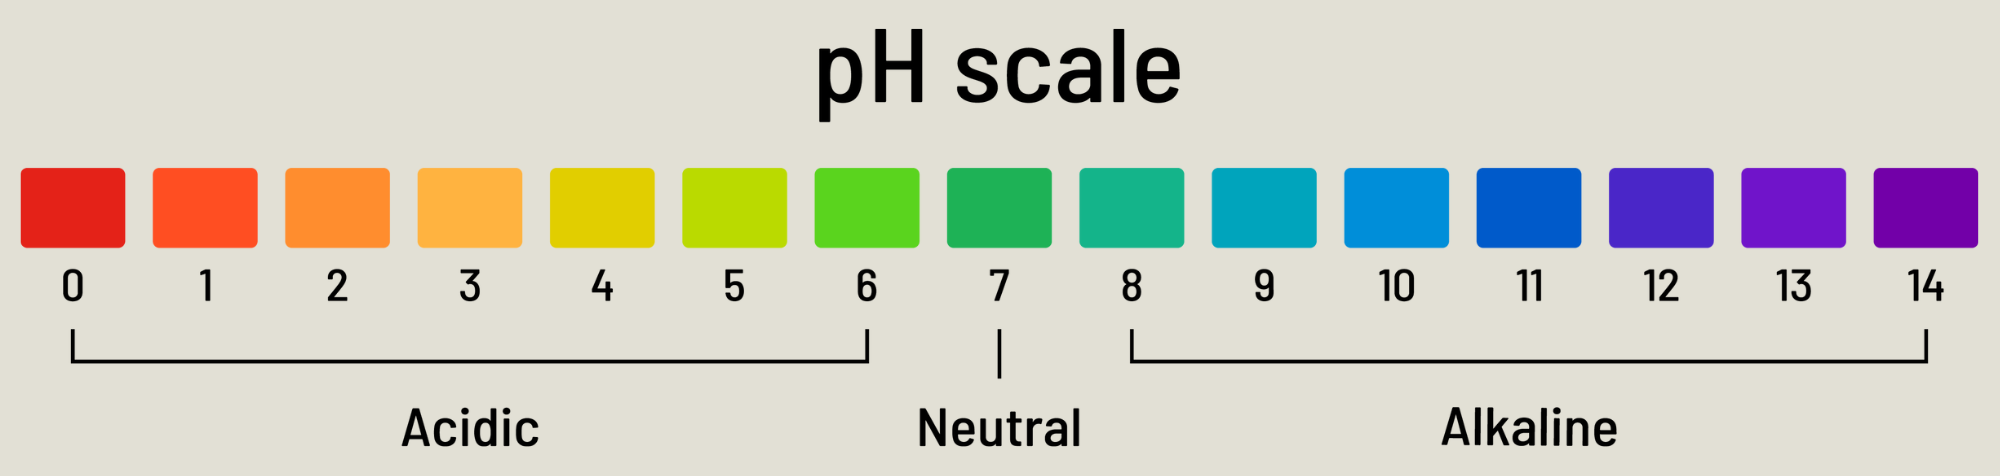
\includegraphics[width=12cm]{Images/anhhoa11/pHscale.png}
		\captionof{figure}{thang pH\label{fig:pHScale}}
		\end{center}
	\end{hopdongian}
\Noibat[][][]{Ý nghĩa pH trong thực tiễn}
\begin{tcolorbox}[
	enhanced jigsaw,
	frame hidden,
	colback=\mycolor!15,
	arc is angular,
	breakable
	]
	Thang đo pH là một công cụ quan trọng để duy trì sự cân bằng và an toàn trong nhiều lĩnh vực của cuộc sống hàng ngày.
\begin{enumerate}
	\item \indam{Kiểm soát chất lượng nước:}
	pH của nước ảnh hưởng đến sự sống của các sinh vật trong nước. Ví dụ, nước có pH quá thấp (acid) có thể gây hại cho cá và các sinh vật thủy sinh. Trong xử lý nước, kiểm tra và điều chỉnh pH là cần thiết để đảm bảo nước an toàn cho con người và động vật.
	\item \indam{Sản xuất thực phẩm và đồ uống:}
	 pH ảnh hưởng đến hương vị, màu sắc và độ an toàn của thực phẩm. Ví dụ, pH của rượu vang, sữa chua và pho mát phải được kiểm soát để đảm bảo chất lượng sản phẩm. Ngoài ra, trong ngành công nghiệp đồ uống, pH còn ảnh hưởng đến sự phát triển của vi khuẩn và quá trình lên men.
	\item \indam{Dược phẩm và y học:}
	pH có vai trò quan trọng trong việc hấp thu và hiệu quả của thuốc. Một số loại thuốc chỉ hoạt động tốt ở một mức pH nhất định, do đó việc điều chỉnh pH của môi trường là cần thiết để đảm bảo thuốc có tác dụng.
	\item \indam{Nông nghiệp:}
	 Đất có pH phù hợp là yếu tố quan trọng đối với sự phát triển của cây trồng. Đất có pH quá cao hoặc quá thấp có thể ảnh hưởng đến khả năng hấp thụ dinh dưỡng của cây. Nông dân thường kiểm tra pH của đất để điều chỉnh phân bón và cải tạo đất.
	\item \indam{Mỹ phẩm:}
	pH của các sản phẩm chăm sóc da và tóc ảnh hưởng đến tính an toàn và hiệu quả của chúng. Các sản phẩm như sữa rửa mặt, dầu gội, và kem dưỡng da cần có pH tương thích với da và tóc để tránh kích ứng và bảo vệ lớp màng acid tự nhiên.
	\item \indam{Xử lý chất thải:}
	pH của chất thải phải được kiểm soát trước khi xả ra môi trường để ngăn ngừa ô nhiễm. Nước thải công nghiệp thường phải được trung hòa pH trước khi xả ra hệ thống thoát nước hoặc sông ngòi.
\end{enumerate}
\end{tcolorbox}
\Noibat[][][]{Chất chỉ thị axit-base}
\vspace{0.5cm}
\begin{tomtat}
	Chất chỉ thị acid - base là chất có màu sắc biến đổi theo giá trị pH của dung dịch.\\
	Một số chất chỉ thị axit-bazo phổ biến:
	\begin{itemize}
		\item Quỳ tím Trong môi trường acid (pH < 7), quỳ tím chuyển sang màu đỏ.Trong môi trường base (pH > 7), quỳ tím chuyển sang màu xanh.
		\item  Phenolphthalein: Chuyển từ không màu (pH < 7) sang hồng (pH > 8.2).
		\item  Methyl orange: Chuyển từ đỏ (pH < 3.1) sang vàng (pH > 4.4).
		\item  Bromothymol blue: Chuyển từ vàng (pH < 6.0) sang xanh dương (pH > 7.6).
	\end{itemize}
\end{tomtat}
\begin{Bancobiet}
	\begin{center}
		\Large\indam{Mối quan hệ giữa pH và màu sắc của hoa cẩm tú cầu}
	\end{center}
	\vspace*{-0.5cm}
	\immini{Hoa cẩm tú cầu (Hydrangea) có thể thay đổi màu sắc dựa trên độ pH của đất nơi chúng được trồng. Sự thay đổi màu sắc chủ yếu được điều chỉnh bởi các hợp chất anthocyanins trong hoa và ion nhôm ($Al^{3+}$) trong đất. 
		\begin{itemize}
			\item Trong đất acid (pH dưới $6.0$): Hoa cẩm tú cầu thường có màu xanh dương.
			\item Trong đất trung tính (pH khoảng $6.0 - 7.0$): Hoa có thể có màu tím nhạt hoặc xanh dương nhạt. 
			\item Trong đất kiềm (pH trên $7.0$): Hoa cẩm tú cầu thường chuyển sang màu hồng hoặc đỏ. 
		\end{itemize}
		}{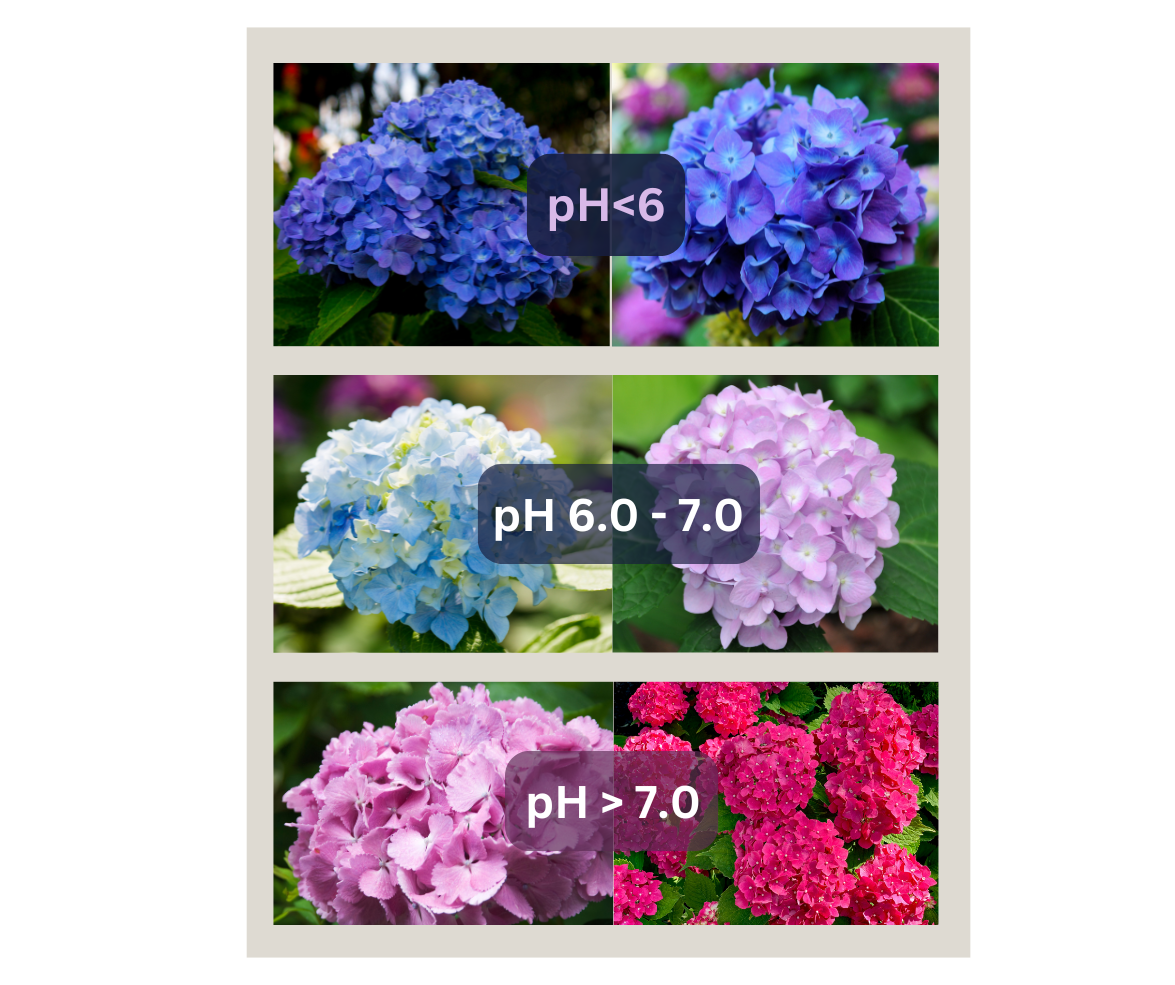
\includegraphics[height=7.5cm,trim={4.2cm 0cm 4.2cm 0cm},clip]{Images/anhhoa11/hoacamtucau.png}}
		Điều chỉnh độ pH của đất có thể giúp thay đổi màu sắc của hoa: thêm các vật liệu làm acid đất như nhôm sulfate để tạo màu xanh dương, hoặc thêm vôi nông nghiệp để làm tăng pH và tạo màu hồng. Các yếu tố khác như loại đất, tình trạng dinh dưỡng và lượng nước cũng ảnh hưởng đến màu sắc của hoa.
\end{Bancobiet}
\subsubsection{Sự thủy phân của muối}
Trong dung dịch nước, một số ion như $\mathrm{Al}^{3+}, \mathrm{Fe}^{3+}$ và $\mathrm{CO}_3^{2-}$ phản ứng với nước tạo ra các dung dịch có môi trường acid/base.
\begin{vidu}
	\begin{enumerate}
		\item Trong dung dịch $\mathrm{Na}_2 \mathrm{CO}_3$, ion $\mathrm{Na}^{+}$ không bị thủy phân, còn $\mathrm{CO}_3^{2-}$ thủy phân trong nước tạo ion $\mathrm{OH}^{-}$ theo phương trình:
		\[
		\mathrm{CO}_3^{2-}+\mathrm{H}_2 \mathrm{O} \rightleftharpoons \mathrm{HCO}_3^{-}+\mathrm{OH}^{-}
		\]
		Vì vậy, dung dịch $\mathrm{Na}_2 \mathrm{CO}_3$ có môi trường base.
		\item Trong dung dịch $\mathrm{AlCl}_3$ và $\mathrm{FeCl}_3$, ion $\mathrm{Cl}^{-}$không bị thuỷ phân, các ion $\mathrm{Al}^{3+}$ và $\mathrm{Fe}^{3+}$ bị thuỷ phân trong nước tạo ion $\mathrm{H}^{+}$theo phương trình ở dạng đơn giản như sau:
		\[
		\begin{aligned}
			& \mathrm{Al}^{3+}+\mathrm{H}_2 \mathrm{O} \rightleftharpoons \mathrm{Al}(\mathrm{OH})^{2+}+\mathrm{H}^{+} \\
			& \mathrm{Fe}^{3+}+\mathrm{H}_2 \mathrm{O} \rightleftharpoons \mathrm{Fe}(\mathrm{OH})^{2+}+\mathrm{H}^{+}
		\end{aligned}
		\]
		Do đó, dung dịch $\mathrm{AlCl}_3, \mathrm{FeCl}_3$ có môi trường acid. Trong thực tế, các loại đất có chứa nhiều ion $\mathrm{Al}^{3+}, \mathrm{Fe}^{3+}$ có giá trị pH thấp hay còn gọi là đất chua. Để khử chua, người ta bón vôi cho đất.
		
		Các muối nhôm và sắt, ví dụ: phèn nhôm $\left(\left(\mathrm{NH}_4\right)_2 \mathrm{SO}_4 \cdot \mathrm{Al}_2\left(\mathrm{SO}_4\right)_3 \cdot 24 \mathrm{H}_2 \mathrm{O}\right)$ và phèn sắt $\left(\left(\mathrm{NH}_4\right)_2 \mathrm{SO}_4 \cdot \mathrm{Fe}_2\left(\mathrm{SO}_4\right)_3 \cdot 24 \mathrm{H}_2 \mathrm{O}\right)$ được sử dụng làm chất keo tụ trong quá trình xử lí nước, dùng làm chất cầm màu trong công nghiệp dệt, nhuộm, hoặc làm chất kết dính, chống nhoè trong công nghiệp giấy,...
	\end{enumerate}
\end{vidu}
\subsubsection{Chuẩn độ acid -base}
Chuẩn độ là phương pháp xác định nồng độ của một chất bằng một dung dịch chuần đã biết nồng độ. Dựa vào thể tích của các dung dịch khi phản ứng vừa đủ với nhau, xác định được nồng độ dung dịch chất cần chuần độ.
\\
Trong phòng thí nghiệm, nồng độ của dung dịch base mạnh (ví dụ NaOH ) được xác định bằng một dung dịch acid mạnh (ví dụ HCl ) đã biết trước nồng độ mol dựa trên phản ứng:
\[
\mathrm{NaOH}+\mathrm{HCl} \longrightarrow \mathrm{NaCl}+\mathrm{H}_2 \mathrm{O}
\]
Khi các chất phản ứng vừa đủ với nhau, số mol HCl phản ứng bằng số mol NaOH .
Ta có:
\[
\mathrm{V}_{\mathrm{HCl}} \cdot \mathrm{C}_{\mathrm{HCl}}=\mathrm{V}_{\mathrm{NaOH}} \cdot \mathrm{C}_{\mathrm{NaOH}}
\]
Trong đó:
	\begin{itemize}
		\item $\mathrm{C}_{\mathrm{HCl}}$ và $\mathrm{C}_{\mathrm{NaOH}}$ lần lượt là nồng độ mol của dung dịch HCl và dung dịch NaOH ;
		\item $\mathrm{V}_{\mathrm{HCl}}$ và $\mathrm{V}_{\mathrm{NaOH}}$ lần lượt là thể tích của dung dịch HCl và dung dịch NaOH (cùng đơn vị đo).
	\end{itemize}
Khi biết $\mathrm{V}_{\mathrm{HCl}}, \mathrm{V}_{\mathrm{NaOH}}$ trong quá trình chuẩn độ và biết $\mathrm{C}_{\mathrm{HCl}}$ sẽ tính được $\mathrm{C}_{\mathrm{NaOH}}$.\\
Thời điểm để kết thúc chuẩn độ được xác định bằng sự đổi màu của chất chỉ thị phenolphthalein.
\subsection{Các dạng bài tập}
\begin{dang}{Tính pH của dung dịch}
\end{dang}
\begin{pp}
	\begin{cacbuoc}
		\item Tính số mol $H^+$ hoặc $OH^-$ trong mỗi dung dịch ban đầu
	\end{cacbuoc}
\end{pp}
\Noibat[][][\faBookmark]{Ví dụ mẫu}
%%%==============VDM1==============%%%
\begin{vd}
	Tính pH của các dung dịch sau:
	\begin{enumerate}
		\item Dung dịch $\mathrm{KOH}$ $0,01\;M$;
		\item Dung dịch $\mathrm{HNO_3}$ $0,1\;M$;
		\item Dung dịch $\mathrm{Ba{(OH)}_2}$ $0,005\;M$;
		\item Dung dịch $\mathrm{H_2SO_4}$ $0,05\;M$.
	\end{enumerate}
	\loigiai{
		\begin{enumerate}
			\item Dung dịch $\mathrm{KOH}$ $0,01\;M$:
			\begin{align*}
				[\mathrm{OH^-}] &= 0,01 \mathrm{M} \\
				\mathrm{pOH} &= -\log[\mathrm{OH^-}] = -\log(0,01) = 2 \\
				\mathrm{pH} &= 14 - \mathrm{pOH} = 14 - 2 = 12
			\end{align*}
			
			\item Dung dịch $\mathrm{HNO_3}$ $0,1\;M$:
			\begin{align*}
				[\mathrm{H^+}] &= 0,1 \mathrm{M} \\
				\mathrm{pH} &= -\log[\mathrm{H^+}] = -\log(0,1) = 1
			\end{align*}
			
			\item Dung dịch $\mathrm{Ba{(OH)}_2}$ $0,005\;M$:
			\begin{align*}
				[\mathrm{OH^-}] &= 2 \times 0,005 = 0,01 \mathrm{M} \\
				\mathrm{pOH} &= -\log[\mathrm{OH^-}] = -\log(0,01) = 2 \\
				\mathrm{pH} &= 14 - \mathrm{pOH} = 14 - 2 = 12
			\end{align*}
			
			\item Dung dịch $\mathrm{H_2SO_4}$ $0,05\;M$:
			\begin{align*}
				[\mathrm{H^+}] &= 2 \times 0,05 = 0,1 \mathrm{M} \\
				\mathrm{pH} &= -\log[\mathrm{H^+}] = -\log(0,1) = 1
			\end{align*}
		\end{enumerate}
	}
\end{vd}
%%%